\subsubsection{任意荷的退化场}\label{degany}

现在，仍在复对称性破缺的情形下，我们将放松所有 $k_a$ 都等于 $1$ 这一限制。
首先考虑单个荷为 $k$ 的 $z$，带有 $q$ 个 Bethe 根。只有当 $k \geq q$ 时 Bethe 方程才有解。
（这一点从 oper 的式 (\ref{normo}) 即可看清。）实际上，根据 Bethe 方程的理论，对给定的 $q$，解是唯一的，并且对应于唯一的针或积分链。

% [Tutor Note: 省略证明] “$k\geq q$ 由 (\ref{normo}) 即可看清”一句略去了论证：按 oper 的次数关系 $p+q=k+1$，$Q$ 的次数就是 Bethe 根数 $q$，故 $P$ 的次数为 $p=k+1-q$；当 $q>k+1$ 时该次数为负，而 $q=k+1$ 时 $P$ 退化为常数、不足以在无穷远处提供 oper 所需的领头行为，因此必须有 $q\le k$。此外“解唯一”是 Bethe 方程理论的一般结论，并非本模型特有。

\begin{figure}
 \begin{center}
     % >>> 原文图 16（原稿第 72 页）
  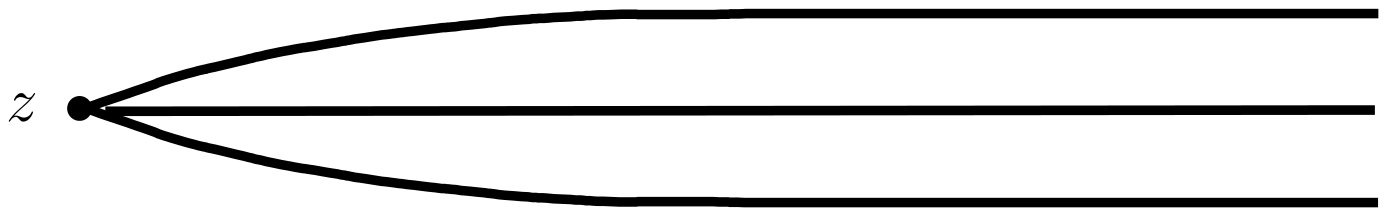
\includegraphics[width=3.5in]{figs/Fig16.png}
 \end{center}
\caption{\small 非最小荷的单个奇异磁单极子的一个积分链。（原稿第 72 页）}
 \label{thimone}
\end{figure}

\begin{figure}
 \begin{center}
     % >>> 原文图 17（原稿第 72 页）
  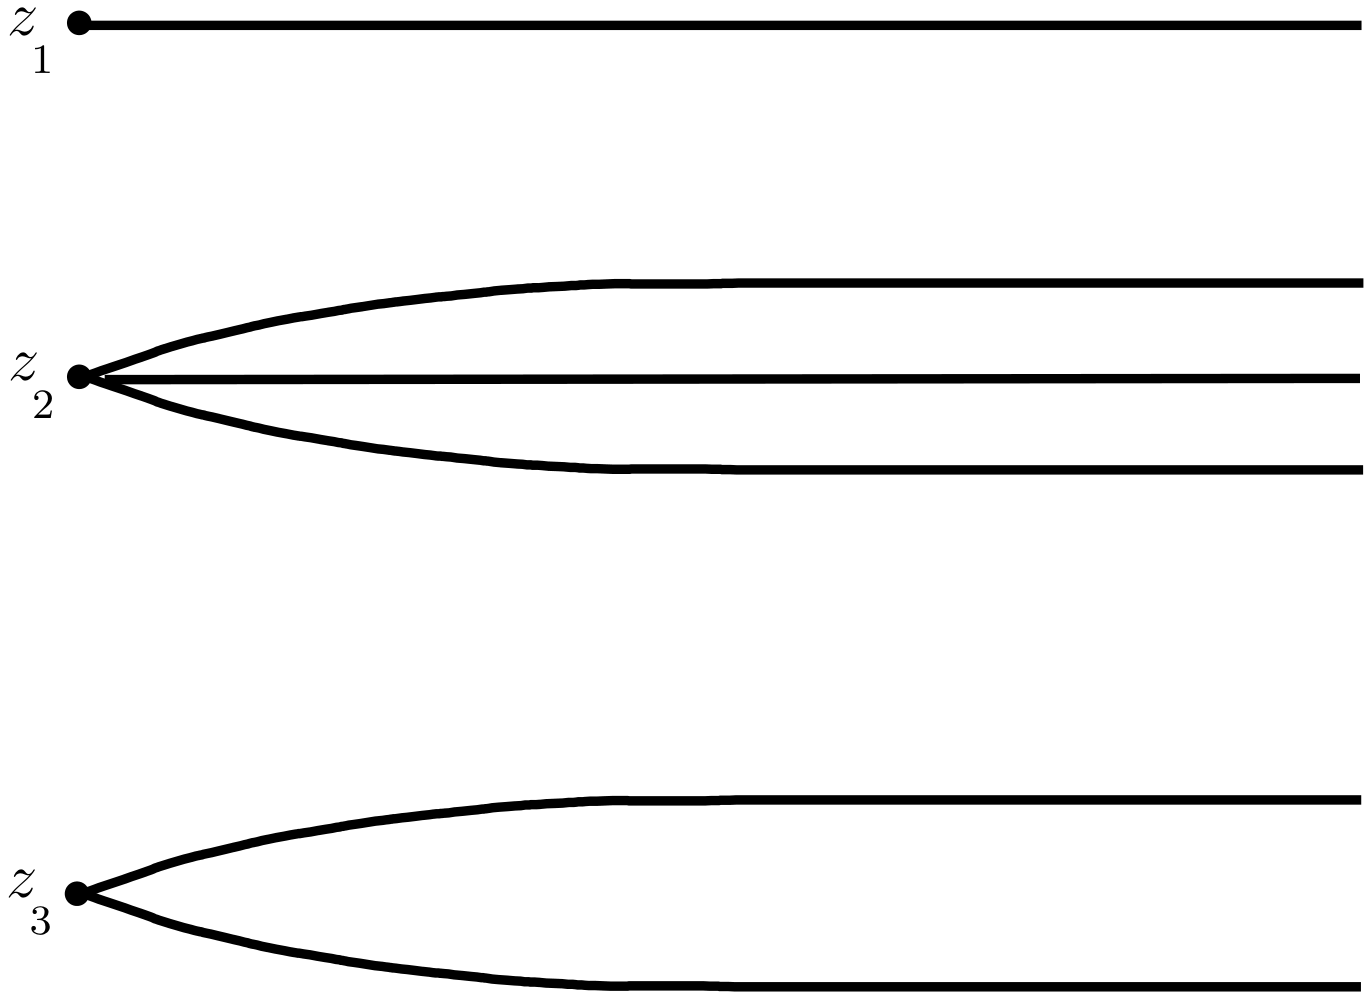
\includegraphics[width=3.5in]{figs/Fig17.png}
 \end{center}
\caption{\small 若干个非最小荷奇异磁单极子的一个积分链。对合适的 $q_a$，我们在 $z_a$ 上附着 $q_a$ 个 $w$。图中 $q_a$ 分别为 $1,3$ 与 2。（原稿第 72 页）}
 \label{thimtwo}
\end{figure}
确实，这个唯一可能的积分链 $\CC^{(q)}$ 很容易描述：把每个 $w_i$ 沿互不相同、互不相交的路径从 $z$ 积分到 $+\infty$，如图~\ref{thimone} 所示。

于是我们可以立即描述最一般情形下的积分链基：$z_a$ 的数目任意，荷为 $k_a$，而 $w_i$ 的数目 $q \leq \sum_a k_a$。对 $q = \sum_a q_a$（其中 $q_a \leq k_a$）的每一种分解方式，我们都得到一条唯一的链：对每个 $a$，把 $q_a$ 个 $w_i$ 沿互不相同、互不相交的路径从 $z_a$ 积分到 $+\infty$，如图~\ref{thimtwo} 所示。这样得到积分链 $\prod_a \CC^{(q_a)}_a$。

在强对称性破缺下（等价地说，当各 $z_a$ 沿虚轴彼此远离时），这些积分链对应于与 Bethe 方程唯一解相伴的针，其中 $q_a$ 个 $w_i$ 位于 $z_a$ 附近。原则上，在此基下导出辫群表示不存在任何障碍。

关于对任意 $k_a$ 构造辫群表示的同调方法（本质上对应于自由场实现），尽管是在没有对称性破缺的情形下，可参见文献~\cite{Ltwo}。

\subsection{关闭对称性破缺}
由于对称性破缺在简化我们的分析方面如此有用，自然就产生了一个问题：需要验证对称性破缺不会影响纽结或链环不变量的取值。

上一节对积分链的描述，只要对称性破缺参数 $c$ 非零就适用。但当 $c\to 0$ 时，我们会失去一些积分链，因为 $w_i$ 不能再趋于无穷。用 $\W$ 的临界点来说，小 $c$ 下的行为容易描述。
对小 $c$，对 Bethe 方程的每个解，Bethe 根自然地分成两个子集。其中 $q_0$ 个 Bethe 根（我们记为 $w^{(0)}_i$，$i=1,\dots,q_0$）在 $c \to 0$ 极限下保持为 $1$ 阶，而其余的 $q_\infty$ 个 Bethe 根（我们记为 $w^{(\infty)}_j,$ $j=1,\dots,q_\infty$）则为 $c^{-1}$ 阶。

在这种情况下，$w^{(0)}_i$ 所满足的 Bethe 方程可由无对称性破缺时相同数目 $w$ 的 Bethe 方程很好地近似。另一方面，$w^{(\infty)}_j$ 所满足的 Bethe 方程可由如下 Bethe 方程很好地近似：有相同数目的 $w$，并且存在单个荷为 $k_{\mathrm{eff}}=\sum_a k_a - 2 q_0$ 的 $z$。式 (\ref{ruy}) 保证 $k_{\mathrm{eff}}$ 非负，因此实际上
 \begin{equation}\label{helpful}0\leq k_{\mathrm{eff}}\leq \sum_ak_a.\end{equation}
正如我们在第~\ref{degany}~节所讨论的，若 $k_{\mathrm{eff}}\geq q_\infty$，则 $w^{(\infty)}_i$ 的 Bethe 方程有唯一解；否则无解。
对所有分解 $q=q_0+q_\infty$ 求和、对 $w^{(0)}_i$ 的 Bethe 方程的所有解求和，最后再对所有可能的 $q$ 值求和，就得到 Bethe 方程解的预期数目 $\prod_{a=1}^d (k_a+1)$。

% [Tutor Note: 易错点] $k_{\mathrm{eff}}=\sum_a k_a - 2q_0$ 中的因子 $2$ 来自 oper 定义里的平方关系 $p(z)Q(z)^2=K(z)$（见前文）：$K$ 的零点总数为 $\sum_a k_a$，而 $Q$ 以平方出现，故留在有限平面的 $q_0$ 个 Bethe 根共消耗 $2q_0$ 个零点，剩下归到无穷远的零点数为 $k_{\mathrm{eff}}$。若漏掉这个 $2$，(\ref{helpful}) 的非负性就会被误判。这一步是本节“关闭对称性破缺”论证的核心记账。

这一计数可以用对偶 $SU(2)$ 规范场论的 Wilson 算符来作如下表述。荷为 $k_a$ 的奇异磁单极子对应于 $SU(2)$ 的表示 $R_a$，其自旋为 $k_a/2$、维数为 $k_a+1$。张量积 $R=\otimes _a R_a$ 的维数为 $\prod_a(k_a+1)$。该表示可以分解为自旋 $k_{\mathrm {eff}}/2$ 的 $SU(2)$ 模的直和（其中 $k_{\mathrm{eff}}$ 受 $0\leq k_{\mathrm{eff}}\leq \sum_ak_a$ 约束，正如 (\ref{helpful}) 中那样）。以该自旋变换的态，其数目等于满足 $\sum_a k_a-2q_0=k_{\mathrm{eff}}/2$ 的 Bethe 方程解的数目（以及对所有可能的 $q$ 值）。

% [Tutor Note: 原文存疑] 此处“满足 $\sum_a k_a-2q_0=k_{\mathrm{eff}}/2$”与本节前面给出的 $k_{\mathrm{eff}}=\sum_a k_a-2q_0$ 相差一个因子 $2$：按上下文，与该自旋对应的应满足 $\sum_a k_a-2q_0=k_{\mathrm{eff}}$（即 $q_0=(\sum_a k_a-k_{\mathrm{eff}})/2$）。原文如此，疑为笔误；按铁律公式未作改动，请读者以后文的计数逻辑为准。

现在考虑各 $z_a$ 的编织。对足够小的 $c$，当穿过一条 Stokes 墙时，存在使 $q_\infty$ 变小的 Morse 流，但不存在使 $q_\infty$ 变大的这类流。原因在于，当 $c\to 0$ 时，Morse 函数 $h=\mathrm{Re}\,\W$ 在临界点处的取值随 $q_\infty$ 增大而增大。（这是因为当 $c\to 0$ 时，$h$ 的某些贡献为 $\ln(1/|c|)$ 阶。借助 (\ref{helpful}) 可以证明，$\ln(1/|c|)$ 的系数是 $q_\infty$ 的增函数。）因此，若按 $q_\infty$ 的取值把物理态空间 $\H$ 分解，则单值性矩阵是分块三角的：
\begin{equation}\label{blocks}B\sim \begin{pmatrix} *& *&* & * & * \cr  *&*&*&*&*\cr
                                                                                   0& 0 & *&* & *\cr 0&0&*&*&*\cr
                                                                         0&0&           0 & 0 & * \cr \end{pmatrix}.\end{equation}
对角块（在所给例子中秩分别为 $2,2,$ 与 1）就是在给定 $q_0=q-q_\infty$ 时、无对称性破缺情形下会有的单值性表示。

只要人们能通过取辫群表示的迹来计算纽结或链环不变量，(\ref{blocks}) 中的非对角块就不重要，因为它们对迹没有贡献。实际上，为了计算 Jones 多项式以及纽结与链环的相关不变量，除了辫群表示之外，还需要一个额外的“融合”操作：产生或湮灭一对荷相同的 $z_a$。要确保纽结不变量不受对称性破缺影响、并且在令 $c=0$ 时不发生变化，我们所需的额外信息是：融合从不涉及在无穷远处产生或湮灭任何 $w$。这一点是自然的，因为融合操作具有局域性。

\subsubsection{一处澄清}\label{clarify}

细心的读者可能注意到这一推导中有一处小小的偷换。不等式 $k_{\mathrm{eff}}\geq 0$ 是由 (\ref{ruy}) 推出的，但 (\ref{ruy}) 最初的推导基于选取 $Q$ 使其次数小于 $P$ 的次数。$c=0$ 时的 Bethe 方程当然存在不满足这一条件的解。我们凭什么可以只考虑这种情形？

设在 $c=0$ 时我们找到一对满足 oper 条件的 $P_0,Q_0$
\begin{equation}\label{opcon} P\frac{\d Q}{\d z}-\frac{\d P}{\d z}Q=K(z).\end{equation}
现在设想开启很弱的对称性破缺。oper 方程变为
\begin{equation}\label{opconz} P\frac{\d Q}{\d z}-\frac{\d P}{\d z}Q-cPQ=K(z).\end{equation}
我们希望随着 $c$ 的开启，存在一对 $(P(z;c),Q(z;c))$ 满足 (\ref{opconz})，并且 $Q$ 具有展开
\begin{equation}\label{turnox}Q(z;c)=Q_0+cQ_1+c^2Q_2+\dots.\end{equation}
这将保证 $Q(z;c)$ 的根在 $c\to 0$ 时趋近于 $Q_0$ 的根，此外还可能有在 $c\to 0$ 时趋于无穷的额外根。人们也许预期 $P$ 会有同样形式的展开，但事实并非如此。满足 (\ref{opcon}) 的多项式 $P,Q$ 的次数 $p$ 与 $q$ 满足 $p+q=k+1$；但一旦 $c\not=0$，该关系就变为 $p+q=k$。因此只要 $c\not=0$，$P$ 的次数就必须下降。其发生方式是：$P$ 的展开实际上是
\begin{equation}\label{nopcon}P(z;c)=c^{-1}P_{-1}+\tilde P_0 +c P_1+\dots\end{equation}
其中我们把 $c^0$ 的系数记为 $\tilde P_0$，因为这个多项式与 $P_0$ 并不相同。把 (\ref{turnox}) 与 (\ref{nopcon}) 代入 (\ref{opconz})，由方程中 $c^{-1}$ 阶的项可知 $P_{-1}$ 是 $Q_0$ 的倍数，且该倍数必须非零，否则方程中 $c^0$ 阶的项将迫使 $p+q\geq k+1$。因此 $p\geq q_0$；再结合 $p+q=k$ 与 $q\geq q_0$，即得 $q_0\leq k/2$，这正是我们想要的。

% [Tutor Note: 含糊点拨] 这一段的关键是“$P$ 在 $c\to0$ 时必须有 $c^{-1}$ 极点”这一反直觉之处：$P,Q$ 本是多项式，但为了在 $c\neq0$ 时把次数总和从 $k+1$ 降到 $k$，$P$ 的系数必须含 $c^{-1}$ 奇性，而这一奇性只能靠 $P_{-1}\propto Q_0$ 来吸收，否则 $c^0$ 阶项会把次数和重新推回 $k+1$。读者若只从“多项式”出发思考，就会卡在此处。

这一分析的教益是：$c=0$ 时确实存在 $q>k/2$ 的 Bethe 方程解，但它们对对称性破缺是不稳定的。这一陈述的各种形式在可积系统文献中为人熟知。

\subsection{三维解释}\label{abdesc}
为了把我们的结果应用于纽结而不只是应用于辫，理解我们迄今所得结果的三维解释会有所帮助。我们考虑 $\R^3$ 中的纽结，因此我们试图在其上求解方程 (\ref{bpseqns}) 的四维流形是 $M_4=\R^3\times \R_+$。我们用欧几里得坐标 $x^1,x^2,x^3$ 描述 $\R^3$。迄今所考虑的绝热演化沿 $x^1$ 方向，而我们已经把其余坐标合并为复变量 $z=x^2+ix^3$。与通常一样，取规范群为 $G=SO(3)$。

我们将集中讨论强对称性破缺的情形。对称性破缺涉及期望值 $\vec\phi=\mathrm{diag}(\vec\ca,-\vec\ca)$ 的选取，其中 $\vec\ca$ 是 $\R^3$ 中的矢量。只要复对称性破缺非零，该矢量就不指向 $x^1$ 方向，即我们为绝热演化所选的方向。从拓扑上看，若两个方向不同，我们不妨把它们视为正交：考虑沿 $x^1$ 方向的绝热演化，并且对称性破缺由 $\vec c = - 2 \vec\ca/\zeta$ 指向正 $x^2$ 方向来描述。按我们迄今的术语，这就是 $c$ 为实正的强复对称性破缺。

我们将只集中讨论各股仅带最小磁荷的情形，因而它们对偶于 $SU(2)$ 的二维表示。在一般时刻，每一股有两个可能的状态：伴随或不伴随一个 Bethe 根 $w_i$。在低能有效阿贝尔规范场论中，若伴随 Bethe 根，则该股带磁荷 1，否则带磁荷 $-1$。

% [Tutor Note: 约定差异] “伴随 Bethe 根则磁荷为 1，否则为 $-1$”这一对应是本文的约定，与后文 $\tilde\CC_1$ 中“Bethe 根伴随 $z_1$，两股荷分别为 1 与 $-1$”一致，但符号本身并无先验理由：它取决于 $\vec c=-\vec\ca/\zeta$ 的方向选择以及 't Hooft 算符荷的正负定义。若采用相反的约定，后文所有 $+/-$ 标记、$\eta$ 的取值与图~\ref{vertexweights} 中的权重都会整体互换，但纽结不变量不变。

当伴随某一股的 Bethe 根移到另一股上时，该股的磁荷就会改变。在绝热演化的语境下，这来自一个 Morse 理论流：Bethe 根从一股移动到另一股。这发生在穿过 Stokes 墙的某个 $x^1$ 值处。第~\ref{twop}~节的教益是：（在强对称性破缺极限下）人们穿过 Stokes 墙的时刻（即 $x^1$ 的某个值），正是两股具有相同 $x^3=\mathrm{Im}\,z$ 值的时刻。因此，Stokes 墙的穿越发生在两股具有相同 $x^1$ 与 $x^3$ 值、从而只在 $x^2$ 上不同的时候。换一种说法，这发生在两股沿对称性破缺方向分开的时候。

\begin{figure}
 \begin{center}
     % >>> 原文图 18（原稿第 76 页）
  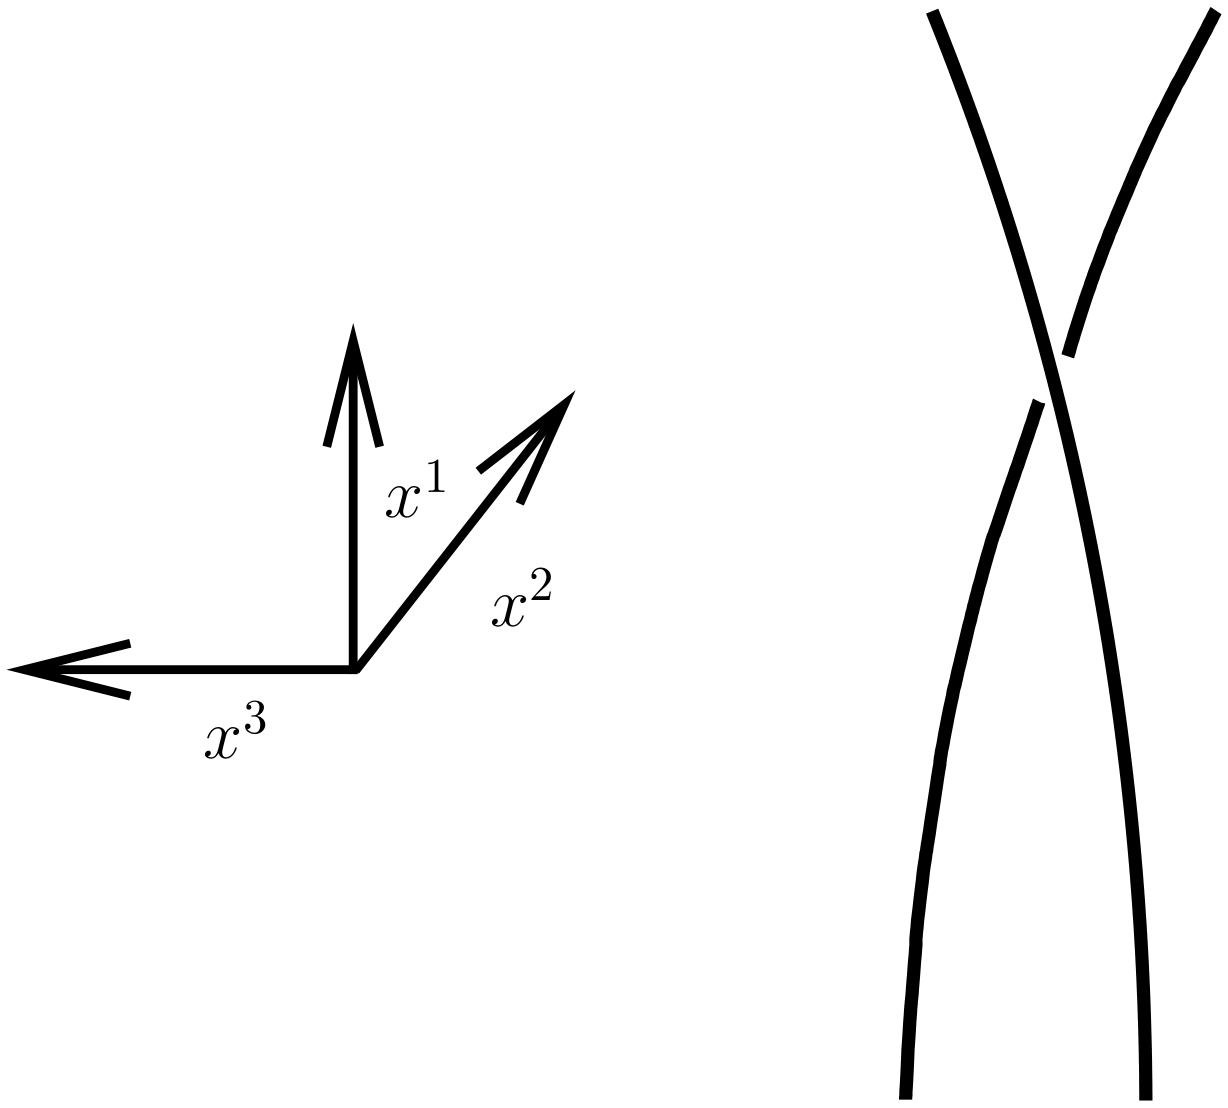
\includegraphics[width=3.5in]{figs/Fig18.png}
 \end{center}
\caption{\small 导致 Morse 理论流的过程的三维图像。图中只画了两股。$x^1$ 方向竖直向上，$x^2$ 方向指向纸内。我们沿负 $x^2$ 轴方向观察此图。坐标 $x^2$ 与 $x^3$ 组合成复变量 $z=x^2+ix^3$。对于复对称性破缺方向的某一特定选择，非平凡 Morse 理论流只能发生在这样的 $x^1$ 值处：两股在该处具有相同的 $x^3$ 值，从而在 $x^1-x^3$ 平面中投影到同一点。用纽结理论的语言来说，我们通过把纽结或链环投影到 $x^1-x^3$ 平面而得到二维图像。在这一投影中会出现交叉点，而非平凡 Morse 流可能发生的位置正是这些交叉点。（原稿第 76 页）\label{crossing}}
\end{figure}

三维图像使问题变得清楚（图~\ref{crossing}）。当两股沿 $x^2$ 方向对齐时，就可能出现 Morse 流。Morse 流发生的时间尺度比绝热演化快得多，因此在绝热图像中它实质上是瞬时的。该流涉及一个 Bethe 根朝正 $x^2$ 方向移动。这种流只能发生在荷相反的股之间，并且只允许正荷朝正 $x^2$ 方向移动。

一般地，给定任意纽结，我们可以有用地把它投影到 $x^1-x^3$ 平面，并从负 $x^2$ 方向观察。我们假定纽结在 $\R^3$ 中的嵌入足够一般，使其切矢量在 $x^1-x^3$ 平面上的投影处处非零；并且纽结到该平面的投影只有简单交叉；最后还假定函数 $x^1$ 沿纽结只有简单的极大值与极小值。一个简单的纽结投影例子见图~\ref{winding}。在这样的纽结投影中，低能阿贝尔描述在离开交叉点处有效，因此在离开交叉点以及局域极大、极小值处（后者我们将在第~\ref{creand}~节讨论），每一股都可以用其磁荷 1 或 $-1$ 来标记。交叉点处荷不变，除非正荷的一股从负荷的一股上方经过，此时可能发生荷交换过程（在 Morse 理论中对应于非平凡梯度流）。

\begin{figure}
 \begin{center}
     % >>> 原文图 19（原稿第 77 页）
  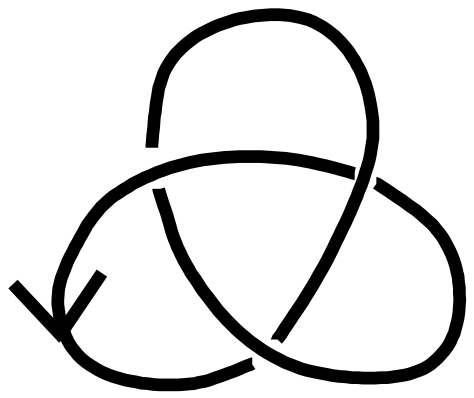
\includegraphics[width=1.2in]{figs/Fig19.png}
 \end{center}
\caption{\small 纽结投影的一个简单例子，其中只有简单交叉以及高度函数的简单极大值与极小值。此图还说明：有向纽结到平面的投影使人们能够定义一个整数不变量 $p=(1/2\pi)\oint\d s \,\d\theta/\d s$，它等于绕纽结一周时纽结切矢量所定义的角 $\theta$ 的总变化量。对图中所示的例子，$p=2$。$p$ 是纽结投影的唯一可以写成沿纽结的局域积分的不变量。它依赖于投影的选取，并非纽结 {\it per se} 的不变量。（原稿第 77 页）}
 \label{winding}
\end{figure}

\begin{figure}
 \begin{center}
     % >>> 原文图 20（原稿第 77 页）
  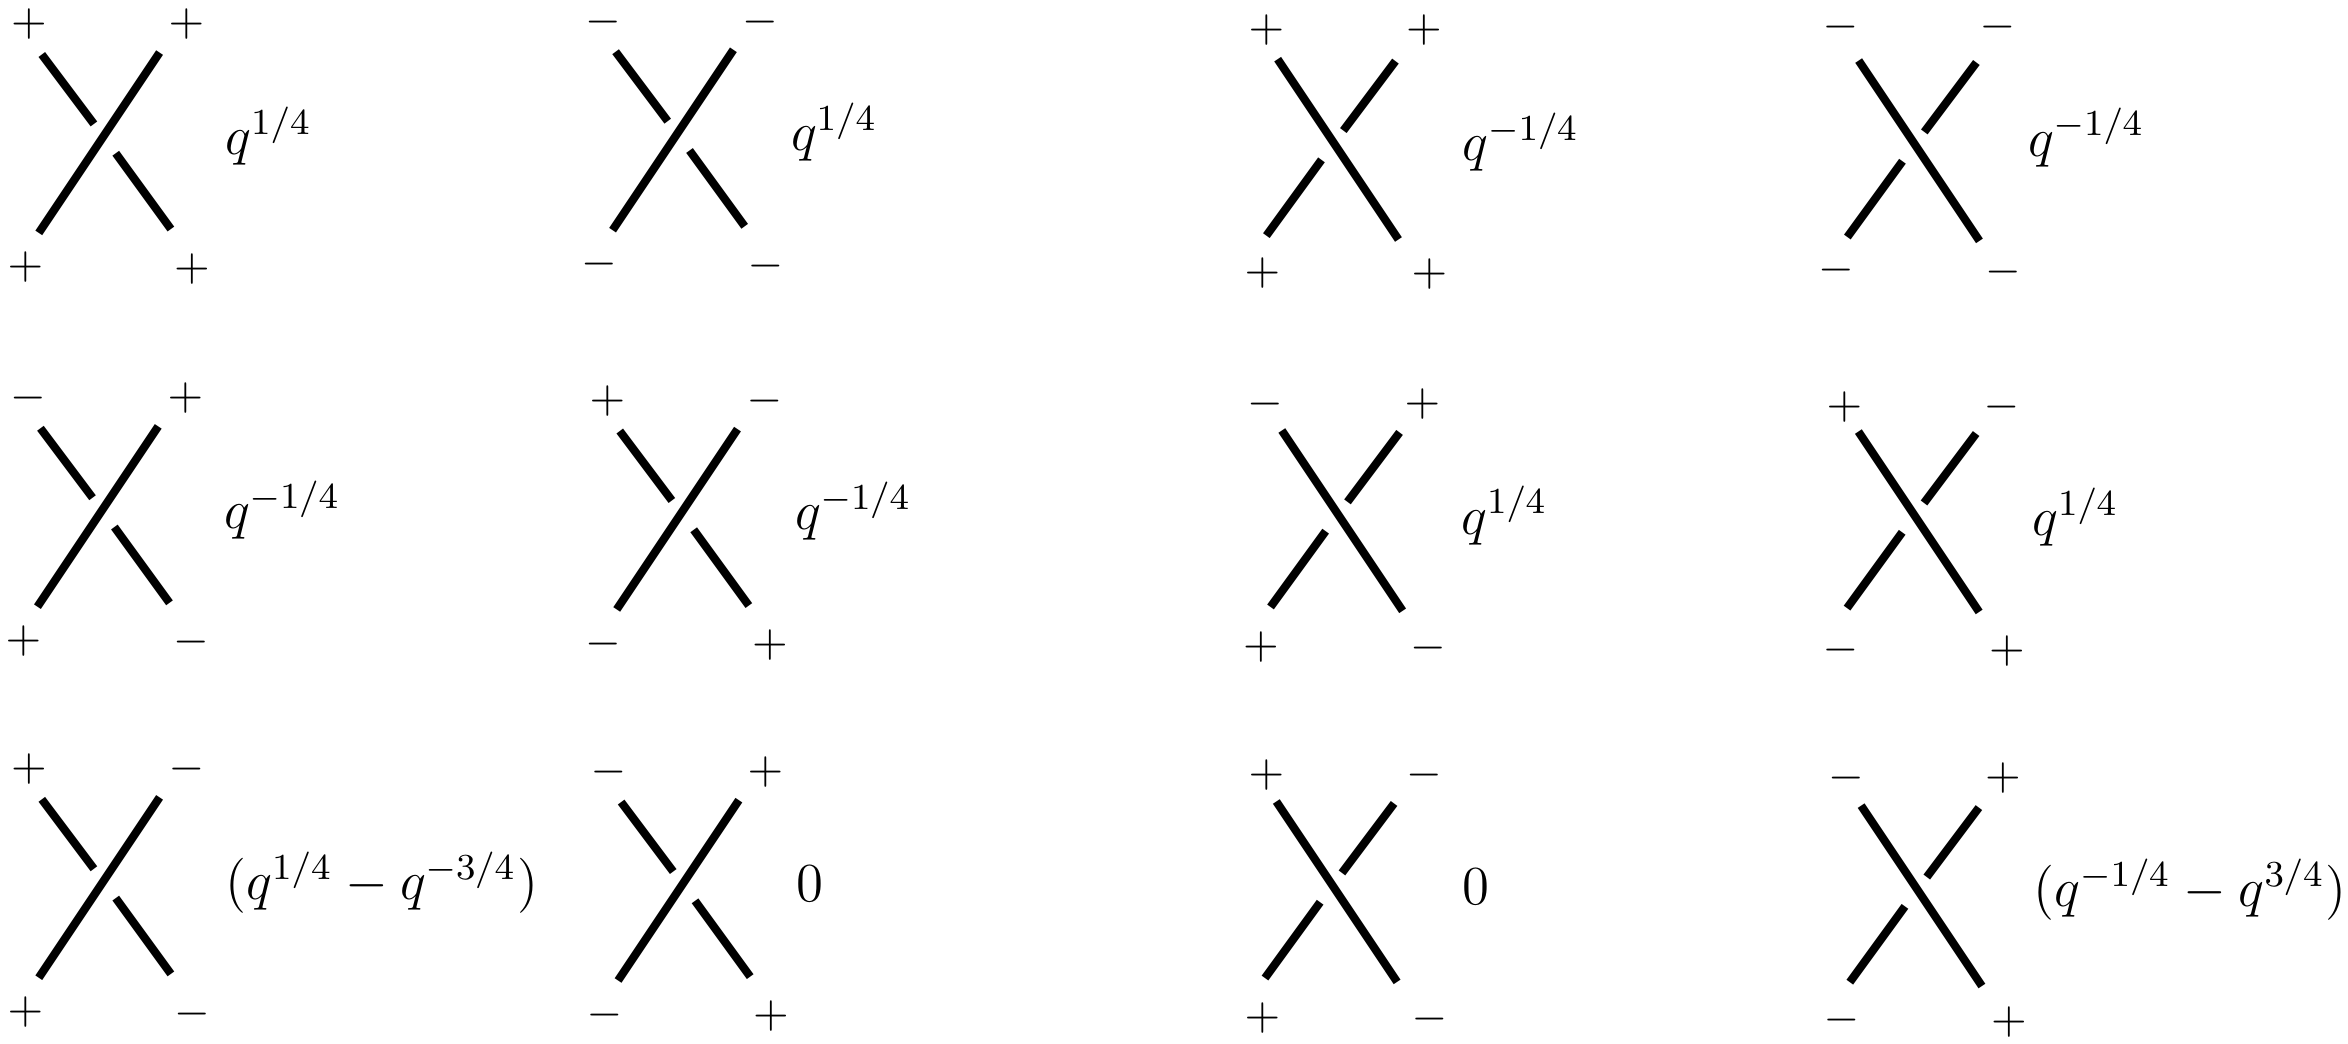
\includegraphics[width=6in]{figs/Fig20.png}
 \end{center}
\caption{\small 顶点模型为两股的每个交叉赋予图中所示的因子。标记各股的 $+$ 与 $-$ 号表示磁荷 $+1$ 或 $-1$ 的向上流动；若把图上下翻转，则只要交换所有 $+$ 与 $-$ 标记，权重保持不变。荷可以在股之间交换，但只有当正荷从底部流入、位于负荷上方时才会发生。若把图左右反射，同时把 $q$ 换成 $q^{-1}$，权重保持不变；这反映了 Chern-Simons 理论在取向反转下的行为。（原稿第 77 页）\label{vertexweights}}
\end{figure}
我们此前的计算为每个可能的交叉赋予一个权重。若交叉处荷不变，这些权重就是 $q^{\pm 1/4}$。当荷发生跳跃时，权重为 $q^{\pm 1/4} - q^{\mp 3/4}$。这些权重总结于图~\ref{vertexweights}。我们已经得到一个已知的顶点模型表示，它表示与 Jones 多项式相伴的辫群表示。
例如可参见文献~\cite{Kauffman} 第 $125$ 页上的 $R$-矩阵（其中 $A$ 就是我们的 $q^{1/4}$），或参见文献~\cite{KauffmanTwo}，特别是第 1777-8 页，或文献~\cite{Vertex} 的图 10。

% [Tutor Note: 易错点] 荷跳跃时的权重 $q^{\pm1/4}-q^{\mp3/4}$ 是两个指数之差，注意后一项是 $3/4$ 而不是 $1/4$；它来自“多出一个 $w$ 的针”与“少一个 $w$ 的针”之间的相对 $q$ 幂次（$q^{1/4}\cdot q^{-1}=q^{-3/4}$）。若把它误写成 $q^{\pm1/4}-q^{\mp1/4}$，顶点模型的 Reidemeister 不变性检验就会失败，这是核对顶点模型权重时最快的自检方式。

\subsubsection{股的产生与湮灭}\label{creand}

为了重现纽结不变量，我们需要理解绝热近似失效的位置，即两股被产生或湮灭的位置。尽管绝热近似在这类点附近失效，低能阿贝尔描述仍然有效。作为一个直接推论，阿贝尔理论中的荷守恒清楚地表明：只能产生或湮灭荷相反的一对股。


从微观理论中的线算符到低能有效描述中的线算符的映射，类似于局域算符的相应映射，但有一点小曲折：系数不是 $c$-数，而是必须沿线输运的量子力学矢量空间。在目前的情形下，这些矢量空间是一维的（在 $U(1)$ 理论中，'t Hooft 算符除其荷之外没有其他结构），但我们仍可从平行输运中得到一个整体因子。这个因子必须沿圈局域地写出，并且必须与拓扑不变性相容。对于没有任何附加结构的纽结，不存在可以写成沿纽结的局域积分的拓扑不变量；但一旦给定纽结到平面（在我们的情形中是 $x^1-x^3$ 平面）的投影，就恰好有一个这样的不变量，即纽结切矢量的总绕数（图~\ref{winding}）。它可以写成 $(1/2\pi)\oint \d s\,\d \theta/\d s$，其中纽结由变量 $s$ 参数化，$\theta$ 是纽结切矢量在 $x^1-x^3$ 平面中的角方向。为定义该不变量的符号，需要纽结的一个取向；在我们的情形中，这来自磁荷的流动方向。当微观 $SU(2)$ 理论在长距离下近似为有效 $U(1)$ 理论时，'t Hooft 算符的有效作用量可能获得一项 $-i\eta\oint \d s \,\d \theta/\d s$，其系数 $\eta$ 是普适的。若纽结的切方向转过角度 $\Delta\theta$，这将贡献一个因子
\begin{equation}
\exp (i\eta \Delta \theta)
\end{equation}
在一对股的产生或湮灭中，切角的变化为 $\Delta\theta=\pi$ 或 $-\pi$，取决于正荷向左还是向右弯折。这一效应会给每个产生或湮灭事件赋予一个普适因子 $\exp(\pm i\pi \eta)$，取决于荷的流动方向。

在相差一个符号的意义下，导致纽结不变量成立的 $\eta$ 的选取是唯一的，即 $\exp(i\pi\eta)=\mp iq^{1/4}$。符号的选择无关紧要，因为每个纽结的产生与湮灭事件数都是偶数；我们将取 $\exp(i\pi\eta)=-iq^{1/4}$。取此 $\eta$ 值时产生与湮灭事件的权重见图~\ref{creation}。$\eta$ 的值或许可以通过研究四维规范场论 BPS 方程在阿贝尔极限附近的行为来直接计算。$q^{1/4}$ 因子应表达在 $SO(3)$ 理论中微观计算的瞬子数与在低能 $U(1)$ 理论中计算的瞬子数之差。$\mp i$ 因子则应涉及 $SO(3)$ 与 $U(1)$ 的费米子行列式之间的比较。整体而言，给定经典解对 Jones 多项式的贡献正比于费米子行列式的符号——这是一个微妙的量，可能接收到微观 $SO(3)$ 理论中带电模的贡献；要把这个符号写成局域因子的乘积，看来必须使用 $i^{\pm 1}$ 这样的因子，而整体符号取决于人们如何把行列式线丛平凡化。

% [Tutor Note: 原文存疑] 本段先写 $\exp(i\pi\eta)=\mp iq^{1/4}$，而两段之后由 (\ref{golf}) 的系数比推出的是 $\exp(i\pi\eta)=\mp i q^{-1/4}$；两处的 $q$ 幂次相反。按后文的推导（比值 $-q^{-1/2}=\exp(2\pi i\eta)$）应有 $\exp(i\pi\eta)=\pm i q^{-1/4}$，故本段开头的 $q^{1/4}$ 疑为笔误。按铁律公式未作改动，请以推导为准。

实际上，$\eta$ 的值可以通过结合阿贝尔描述中可得的信息与共形块描述中可得的信息来推出。当一对股被产生或湮灭时，我们预期它们融合为恒等场。这意味着位于 $z_1$ 与 $z_2$（比如）处的两条邻近的股伴随一个 Bethe 根 $w$，而该 Bethe 根的积分链是连接 $z_1$ 与 $z_2$ 的针 $\CC_{12}$。另一方面，在第~\ref{twop}~节中我们还定义了积分链 $\tilde \CC_1$ 与 $\tilde \CC_2$，其性质是 $z_1$ 处与 $z_2$ 处的股具有确定的磁荷。（例如，在 $\tilde \CC_1$ 中 Bethe 根伴随 $z_1$，因此两股的荷分别为 1 与 $-1$。我们按 $x^3=\mathrm{Im}\,z$ 递减的次序排列 $z_1$ 与 $z_2$。）这些链之间的关系为
\begin{equation}\label{golf}\CC_{12}=\CC_1-\CC_2=q^{-1/4}\tilde\CC_1-q^{1/4}\tilde \CC_2.
\end{equation}
产生一对荷 $(1,-1)$ 的振幅与产生一对荷 $(-1,1)$ 的振幅之比，等于 (\ref{golf}) 右端系数之比，即 $-q^{-1/2}$。另一方面，在阿贝尔描述中该比值为 $\exp(2\pi i\eta)$。于是 $\exp(i\pi\eta)=\mp i q^{-1/4}$，如图~\ref{creation} 所示。



\begin{figure}
 \begin{center}
     % >>> 原文图 21（原稿第 79 页）
  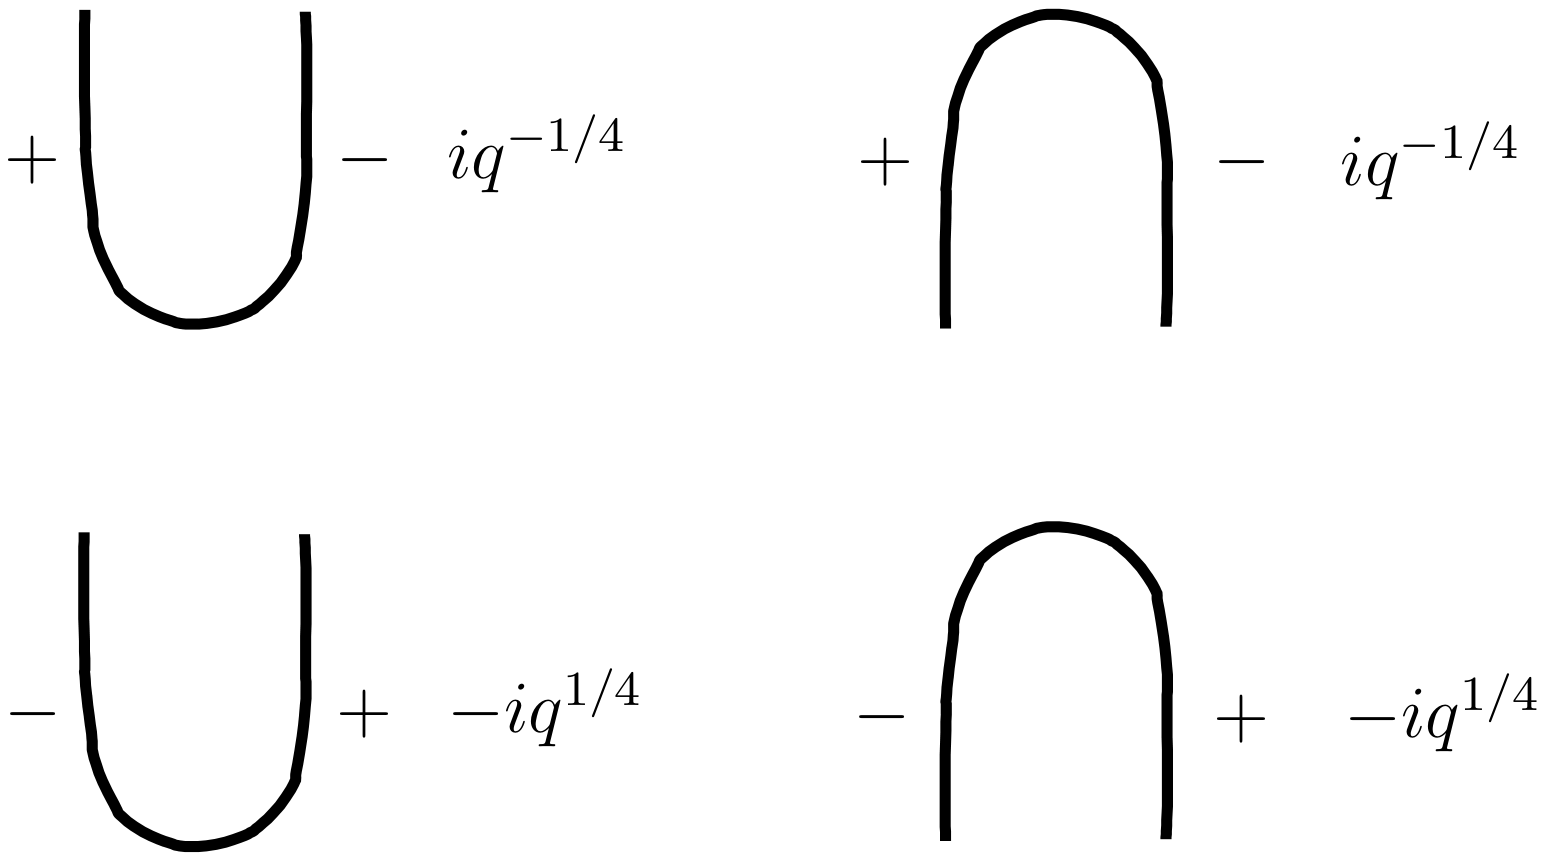
\includegraphics[width=4in]{figs/Fig21.png}
 \end{center}
\caption{\small 一对股产生或湮灭时顶点模型的权重。如图~\ref{vertexweights} 那样，若交换 $+$ 与 $-$ 标记，则权重在把图上下翻转时不变；若把 $q$ 换成 $q^{-1}$，则权重在左右反射下不变。（原稿第 79 页）\label{creation}}
\end{figure}

我们已经得到了本质上标准的、用于计算 Jones 多项式的顶点模型算法：给定一个纽结或链环，选取它到 $x^1- x^3$ 平面的投影，使得投影中只有简单交叉，且函数 $x^1$ 只有简单的极大值与极小值。把链环分成由极大值、极小值与交叉点分隔的线段。用 $\pm$ 标记各线段，并对所有标记求和，每个标记以交叉点、极大值与极小值处局域权重的乘积加权。
稍后我们会给出一些简单的例子。
